\chapter{The Central Limit Theorem and Experimental Uncertainties}

%
% TODO:  Students were confused about how to handle bin position
% for plotting discrete data...  some clarification (text, figures) is needed.
%

\section{Introduction}

In this lab, you will produce a numerical demonstration of the central
limit theorem.  You will also model the propagation of uncertainties
and compare with the calculated uncertainties. For this lab there are only jupyter notebook entries. 


\section{Sampling Distributions}

\begin{figure}[htbp]
\begin{center}
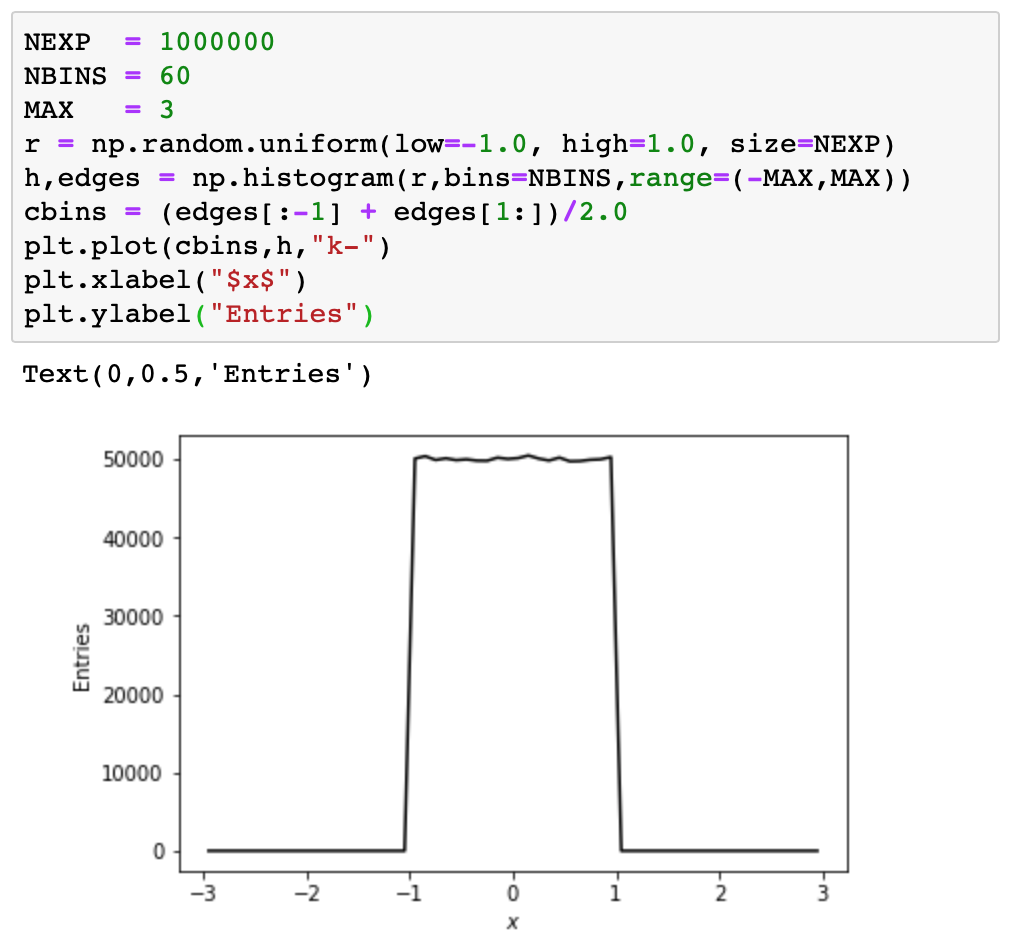
\includegraphics[width=0.75\textwidth]{figs/labs/uncertainties/step.png}\\
\end{center}
\caption{\label{fig:samplingstep} Sampling from the uniform distribution. }
\end{figure}

\begin{figure}[htbp]
\begin{center}
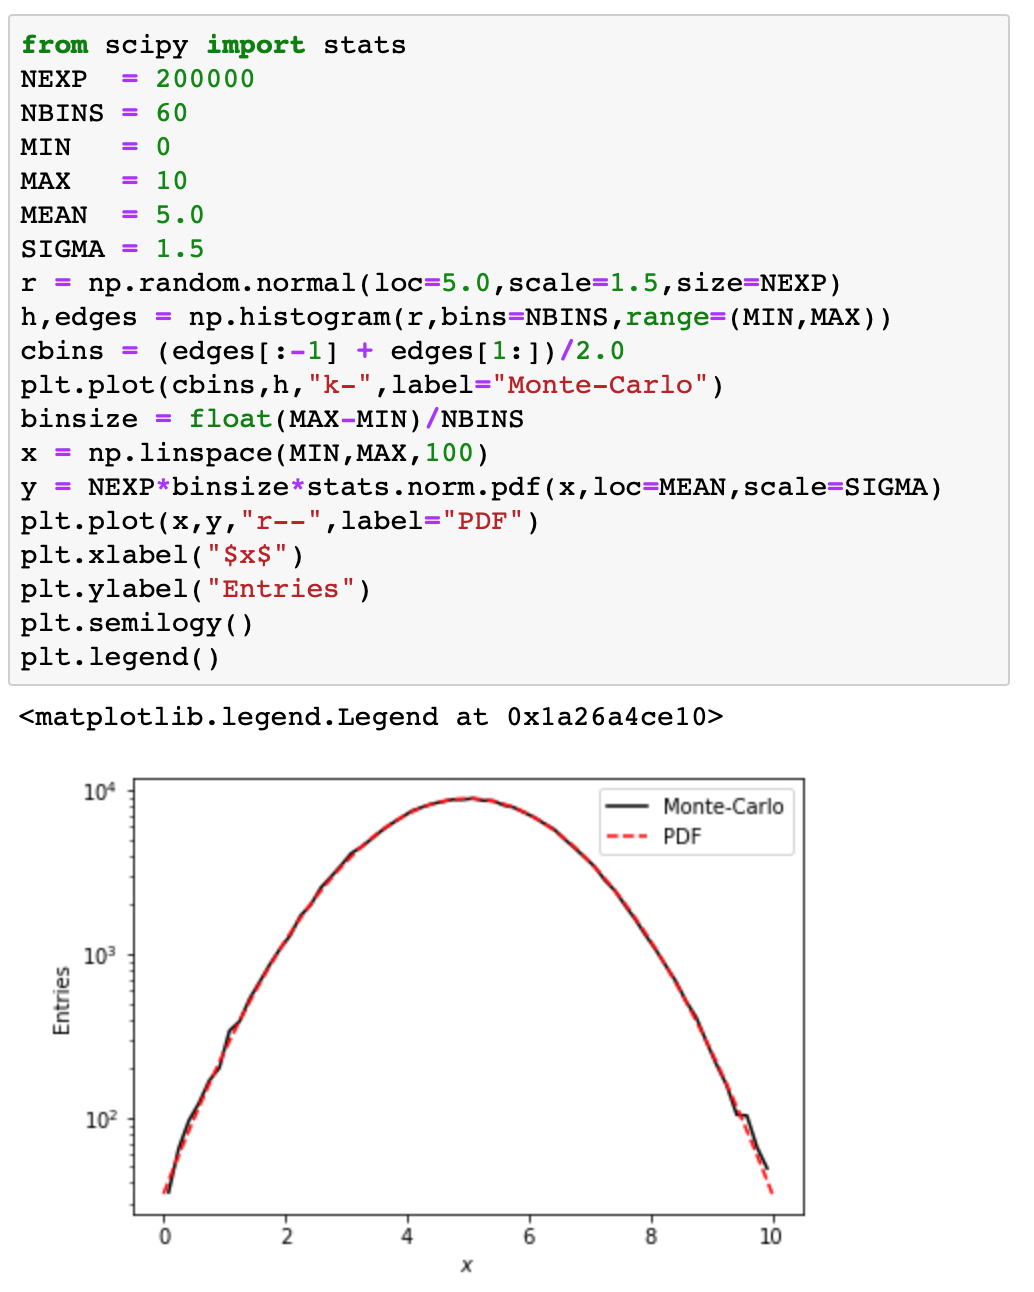
\includegraphics[width=0.75\textwidth]{figs/labs/uncertainties/gaussian.png}\\ 
\end{center}
\caption{\label{fig:samplinggauss} Sampling from the Gaussian distribution and comparison with the Gaussian PDF.}
\end{figure}

Scientific python provides functions to draw random samples according
to various distributions.  In today's lab, we will draw samples
uniformly in the interval $[-1,1]$, as demonstrated in Fig.~\ref{fig:samplingstep}.   The line
\begin{verbatim}
r = np.random.uniform(low=-1.0, high=1.0, size=NEXP)
\end{verbatim}
creates a NumPy array {\tt r} which contains {\tt NEXP} entries, with
each entry chosen uniformly and randomly in the range from -1 to 1.
In the example, these events are displayed in a histogram.  When
plotting histograms with plenty of statistics (one million entries
here) and fine binning (60 bins here) it is usually preferable to use
lines instead of points with error bars for plotting the histograms,
as is done in this example.  Notice, however, that even with one
million events, there are still statistical fluctuations which prevent
the curve from being perfectly smooth.

In Fig.~\ref{fig:samplinggauss}, entries are instead drawn from the Gaussian distribution with the line:
\begin{verbatim}
r = np.random.normal(loc=5.0,scale=1.5,size=NEXP).
\end{verbatim}
The histogram is plotted with a logarithmic $y$ scale:
\begin{verbatim}
plt.semilogy()
\end{verbatim}
which results in the Gaussian distribution appearing as a parabola.  The histogram is compared to the Gaussian PDF appropriately normalized:
\begin{verbatim}
x = np.linspace(MIN,MAX,100)
y = NEXP*binsize*stats.norm.pdf(x,loc=MEAN,scale=SIGMA)
\end{verbatim}


\section{Demonstration of the Central Limit Theorem}

In this section, you'll show that average value of random variables
chosen uniformly from -1 to 1 approaches a Gaussian distribution,
consistent with the central limit theorem.  First create a 2-D array
of size {\tt NEXP} by {\tt NAVG} filled with uniform random values in
the interval from -1 to 1, as follows:
\begin{verbatim}
r = np.random.uniform(low=-1.0, high=1.0, size=(NEXP,NAVG))
\end{verbatim}
Then calculate averages values from {\tt NAVG} entries:
\begin{verbatim}
x = np.sum(r, axis=1)/float(NAVG)  
\end{verbatim}
From the Central Limit Theorem, we expect the entries in x to approach a Gaussian distribution.

\begin{plot}  Set {\tt NEXP} to 1000000 for plenty of statistics.
Produce three different histograms with 40 bins covering the range
from -1.2 to 1.2 for three values {\tt NAVG}: 1,2, and 3.  Plot all
three histogram in the same graph with appropriate legend. \end{plot}

Your plot will show that already for three contributions to the average, the result looks quite Gaussian on a linear scale.  For more precise comparison, will use a log scale and compare to the PDF.

\begin{plot} Calculate {\tt NEXP}$=1000000$ average values {\tt x} for {\tt NAVG}$=10$.  Calculate the mean value of the entries in {\tt x} using the {\tt np.mean} function.  Calculate $\sigma$ for the entries in $x$ by taking the square root of the output from the {\tt np.var} (variance) function.  Produce a histograms with 20 bins covering the range
from -0.5 to 0.5 for the average values.  Compare with a Gaussian distribution, appropriately normalized, using your calculated values from the  mean and sigma.  Plot both the histogram and PDF on the same graph, including an appropriate legend.  Use a logarithmic $y$ axis. \end{plot}


\section{Propagation of Uncertainties}

\begin{figure}[htbp]
\begin{center}
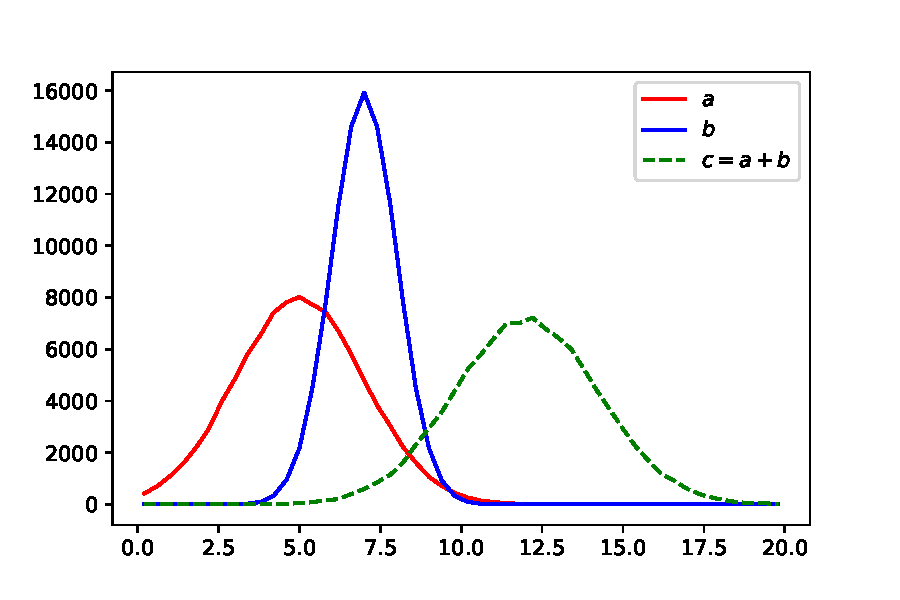
\includegraphics[width=0.75\textwidth]{figs/labs/uncertainties/addunc.pdf}\\
\end{center}
\caption{\label{fig:addunc} Simulation of many measurements of the quantity $c = a + b$. }
\end{figure}

Consider two measured values $a \pm \sigma_a$ and $b \pm \sigma_b$.  If we calculate the quantity $c = a + b$ or $c = a - b$, the uncertainty on the calculated value $c$ is given by:
\begin{displaymath}
\sigma_c = \sqrt{\sigma_a^2 + \sigma_b^2}.
\end{displaymath}
If instead, we calculate $c = a * b$ or $c = a/b$ the fractional uncertainty on $c$ is given by:
\begin{displaymath}
\frac{\sigma_c}{c} = \sqrt{\left(\frac{\sigma_a}{a}\right)^2 + \left(\frac{\sigma_b}{b}\right)^2}.
\end{displaymath}
In this section, you'll develop a numerical simulation for the
propagation of uncertainties under addition, subtraction,
multiplication, and division.  An example, for $c = a + b$ is shown in Fig.~\ref{fig:addunc}.

\begin{print} Pick values for $a$, $b$, $ \sigma_a$ and $ \sigma_b$ for simulating subtraction: $c=a-b$. Print them out in your notebook. Choose the values that are different from what is plotted in Fig.~\ref{fig:addunc}.  \end{print}

\begin{plot} 
Simulate the measurement $a$ by drawing 100,000 random variables
sampled from the Gaussian distribution with mean $a$ and sigma
$\sigma_a$, and likewise for $b$.  Calculate the values of $c = a -b $ from
the $a$ and $b$ values.  Plot the result in histogram with 50 bins and an appropriate range. \end{plot} 

\begin{print} 
Calculate the mean and variance of the mean and variance of the simulated $c$ values and compare to your expectations for the mean, variance of the distribution and variance of the mean. Apply the standard propagation of uncertainties for calculating expectation value for the variances. 
 \end{print}


This is a \textbf{sign-off point} for this lab. 

\begin{print} Pick values for $a$, $b$, $ \sigma_a$ and $ \sigma_b$ for simulating division: $c=a/b$. Print them out in your notebook.  Choose the values that are different from what is plotted in Fig.~\ref{fig:addunc}.  \end{print}

\begin{plot} 
Simulate the measurement $a$ by drawing 100,000 random variables
sampled from the Gaussian distribution with mean $a$ and sigma
$\sigma_a$, and likewise for $b$.  Calculate the values of $c = a/b $ from
the $a$ and $b$ values.  Plot the result in histogram with 50 bins and an appropriate range. \end{plot} 

\begin{print} 
Calculate the mean and variance of the mean and variance of the simulated $c$ values and compare to your expectations for the mean, variance of the distribution and variance of the mean. Apply the standard propagation of uncertainties for calculating expectation value for the variances. 
 \end{print}

 
%{\bf Plot 3-6:}  Produce four plots simulating addition, subtraction, multiplication, and division, as in Fig.~\ref{fig:addunc}.  In each case, compare the measured variance of the $c$ values with your expectation.






























